%% -*- coding:utf-8 -*-

\chapter{Lexical Functional Grammar}
\label{Kapitel-LFG}


Lexical Functional Grammar (LFG) was developed in the 80s by Joan Bresnan and Ron Kaplan \citep{BK82a}. LFG forms part of
so"=called West-Coast linguistics: unlike MIT, where Chomsky works and teaches, the institutes of researchers such as Joan
Bresnan and Ron Kaplan are on the west coast of the USA (Joan Bresnan in Stanford and Ron Kaplan at Xerox in Palo Alto and now at the language technology firm
Nuance Communications in the Bay Area in California).


\citet{BK82a} view LFG explicitly as a psycholinguistically plausible alternative to transformation"=based approaches. For a discussion of
the requirements regarding the psycholinguistic plausibility of linguistics theories, see Chapter~\ref{Abschnitt-Diskussion-Performanz}. 

The more in"=depth works on German are \citew{Berman96a-u,Berman2003a} and \citew{Cook2001a}.

LFG has well-designed formal foundations \citep{KB82a-u,Kaplan95a}, and hence first implementations
were available rather quickly \citep*{FR83b,FR83a,Yasukawa1984a-u,BH86a-u,%
ED86a-u,% CHARON Parser
WA86a-u,%
Delmonte90a-u,% Italien
HHP91a-u,% Chinesisches kommerzielles System
Kohl92a-u,KGPRM92a-u,% ACORD project CHARON Generator
KM96a-u,%
Mayo97a-u,Mayo99a-u,%Konstanzer system
BS2005b-u,BS2005a-u,%SxLFG
Clement2009a-u,CK2001a-u% XLFG
}. 

The following is a list of languages with implemented LFG fragments, probably incomplete:
% Tracy 30.03.2010
%
% Hungarian is just starting in ParGram and so does not have any
% papers on the implementation.  Welsh does not have a good citation for
% the implemented grammar.  Spanish ParGram is only a toy grammar and
% has no publications.
%
% Lionel Clement (cc-ed here, hopefully with his correct address) has
% an LFG implementation which you might wish to include.  It has a web
% interface which makes it particularly nice for teaching.
%
% http://www.xlfg.org/
%
% Leonel de Alencar, 31.03.2010
% Es gibt tatsächlich viele ältere LFG-Systeme. Meines Wissens ist das in SWI-Prolog implementierte
% GFU-Lab das einzige, das noch funktioniert. Dieses System, das sich gut für den Unterricht eignet,
% ist aber kein orthodoxes LFG-System und z.B. mit LKB nicht vergleichbar.
%
% AdamP 25.05.2015 zu ParGram
%% . Hungarian
%% • Norwegien
%% • Urdu
%% • Wolof
%% • Turkish 
%% • Polish
%% • Georgian (toy grammar? – not sure)
%% • Slovenian (toy grammar? – not sure)
%% • Greek (rather preliminary work at the moment)
%% • German (not sure about current developments)
%% • English (not developed for some time)
%% • French (not developed for a long time)



\begin{itemize}
\item Arabic\il{Arabic} \citep{Attia2008a-u},
\item Arrernte\il{Arrernte} \citep*{Dras2012a-u},
\item Bengali\il{Bengali} \citep{SC97a-u},
%\item Chinese\il{Mandarin Chinese}
\item Danish\il{Danish} \citep{Oersnes2002b-u,OW2003a-u,OW2004a-u},
\item English\il{English} \citep*{HHP91a-u,BDFK99a-u,RKKCMJ2002a-u,KM2007a-u},
\item French\il{French} \citep*{Zweigenbaum91a-u,Frank96b-u,FZ2002a-u,BDFK99a-u,CK2001a-u,BSL2005a-u,SdA2016a-u,Alencar2017a-u},
% Knueppel2001a-u
%
%
\item Georgian\il{Georgian} \citep{Meurer2009a-u},
\item German \citep{Rohrer96a,Berman96a-u,KR97a-u,BDFK99a-u,Dipper2003a-u,RF2006a,Forst2006a-u,Frank2006a-u,FR2009a-u},
%\item Griechisch\il{Griechisch},
\item Hungarian\il{Hungarian} \citep{LRT2010a-u},
\item Indonesian\il{Indonesian} \citep*{AADMS2009a-u},
\item Italian\il{Italian} \citep*{Delmonte90a-u,Mayo99a-u,Quaglia2012a-u},
\item Irish\il{Irish} \citep{Sulger2009a-u,Sulger2010a-u},
\item Japanese\il{Japanese} \citep*{HHP91a-u,MO2003a-u,Umemoto2006a-u},
\item Korean\il{Korean} \citep*{HHP91a-u},
\item Malagasy\il{Malagasy} \citep*{Randriamasimanana2006a-u,DLM2006a-u},
\item Mandarin Chinese\il{Mandarin Chinese} \citep*{HHP91a-u,FK2007a-u},
\item Murrinh-Patha\il{Murrinh-Patha} \citep{SN2012a-u},
\item Norwegian\il{Norwegian} \citep*{DMR2005a},
\item Polish\il{Polish} \citep*{PP2012a-u},
\item Portuguese\il{Portuguese} \citep{Alencar2004a-u,Alencar2013a-u,Alencar2015a-u},

% Tracy: Toy
% Forst:
% Apart from that, I have a little Spanish grammar, but it's very phenomenon-driven, not broad-coverage by any means and not documented anywhere, let alone in publications. 
\item Spanish\il{Spanish} \citep{Mayo99a-u},
%
% klein?
%\item Thai
\item Tigrinya\il{Tigrinya} \citep{Kifle2012a-u},
\item Turkish\il{Turkish} \citep{CO2006a-u},
\item Hungarian\il{Hungarian} \citep*{LRT2010a-u,RLC2011a-u},
% Journal-Artikel, aber unklar ob implementiert
\item Urdu/Hindi\il{Urdu}\il{Hindi} \citep*{BHKR2007a-u,BBS2008a-u},

% Forst: nichts mehr gehört
%\item Vietnamesisch\il{Vietnamesisch}
\item Welsh\il{Welsh} \citep{MS2005a-u}
and
\item Wolof\il{Wolof} \citep{Dione2012b-u,Dione2013a-u}.
\end{itemize}
Many of theses grammars were developed in the ParGram consortium\footnote{%
  \url{http://pargram.b.uib.no/research-groups/}. 2018-02-20.
} \citep*{BKNS99a-ed,BDKMR02a-u}. Apart from these grammars there is a small fragment of Northern
Sotho\il{Northern Sotho}, which is currently being expanded \citep{Faasz2010a-u}. 

%Im ParGram"=Projekt wird angestrebt, alle Sprachen mit den gleichen funktionalen Strukturen zu
%analysieren. Die Konstituentenstruktur wird als einzelsprachlich  angesehen

Many of the LFG systems combine linguistically motivated grammars with a statistical
component.\is{statistics} Such a component can help to find preferred readings of a sentence first,
it can increase the efficiency of processing and make the complete processing robust (for instance
\citealp{KRKMVC2004a-u,RKKCMJ2002a-u}). Josef van Genabith's group in Dublin is working on the induction of
LFG grammars from corpora (\eg \citealp{JGCCR99a-u,DBCGW2005a-u,CBFDRCW2005a-u,CG2006a-u,GWG2007a-u,CBDRGW2008a-u,SG2009a-u}). 

\pagebreak
Some of the systems can be tested online:
\begin{itemize}
\item \url{http://iness.uib.no/xle-web/xle-web}

% Statistik Dublin
%\item \url{http://lfg-demo.computing.dcu.ie/lfgparser.html}
\item \url{http://www.xlfg.org/}
\end{itemize}




\section{General remarks on the representational format}
\label{Abschnitt-Format-LFG}

LFG assumes multiple levels of representation.\footnote{%
	The English examples and their analyses discussed in this section are taken from
        \citet{Dalrymple2001a-u} and \citet{Dalrymple2006a}.
} The most important are c"=structure\is{c"=structure} and f"=structure\is{f"=structure}. c"=structure is the constituent
structure and it is licensed by a phrase structure grammar. This phrase structure grammar uses
\xbar~structures for languages for which this is appropriate. f"=structure stands for functional structure. Functional structure contains information about the predicates involved
and about the grammatical functions (subject, object, \ldots) which occur in a constituent. Mappings
mediate between these representational levels.


\subsection{Functional structure}

In LFG, grammatical functions such as subject and object play a very important role. Unlike in most other theories discussed in this book, they are primitives
of the theory. A sentence such as (\mex{1}a) will be assigned a functional structure as in (\mex{1}b):


\eal
\ex David devoured a sandwich.
\ex \lfgms{ pred & `DEVOUR\sliste{\lfgsubj, \lfgobj}'\\
         subj & \lfgms{ pred &  `DAVID' \\
                   }\\
         obj  & \lfgms{ spec & A\\
                     pred & `SANDWICH'\\
                   }\\
       }
\zl

\noindent
All lexical items that have a meaning (\eg nouns, verbs, adjectives) contribute a \textsc{pred}\isfeat{pred} feature with a corresponding value.
The grammatical functions governed by a head (government = subcategorization)
are determined in the specification of \textsc{pred}.\footnote{%
In the structure in (\mex{0}b), the \lfgsubj{} and \lfgobj{} in the list following \emph{devour} are identical to the values of \lfgsubj{} and \lfgobj{} in the structure. For reasons of presentation, this will not be explicitly indicated in this structure and following structures.
}
Corresponding functions are called \emph{governable grammatical functions}\is{grammatical function!governable}. Examples of this are shown in Table~\vref{Tabelle-GOV} \citep{Dalrymple2006a}.
\begin{table}
\centering
\begin{tabular}[t]{@{}lp{26em}@{}} 
\lsptoprule
\textsc{subj}\isfeat{subj}: & subject \\ 
%
\textsc{obj}\isfeat{obj}: & object\\ 
%
\textsc{comp}\isfeat{comp}: & sentential complement or closed (non-predicative) infinitival complement\\
\textsc{xcomp}\isfeat{xcomp}: & open (predicative) complement, often infinitival, the \textsc{subj} function
is externally controlled\is{control}\\
\objtheta: & secondary \textsc{obj} functions that are related to a special, language \\
           & specific set of grammatical roles; English has \objtheme only.\\
%
\obltheta: & a\isfeat{obl} group of thematically restricted oblique functions, as for instance
         {\obl\downlett{GOAL}} or {\obl\downlett{AGENT}}. These often correspond to adpositional
         phrases in c-structure.\\
\lspbottomrule
\end{tabular}
\caption{\label{Tabelle-GOV}Governable grammatical functions}
\end{table}\todostefan{\objtheta im Deutschen?}%
The \pred specification corresponds to the theta grid\is{theta-grid@$\theta$-grid} in \gbt. The valence\is{valence} of a head is specified by
the \predv.

The non"=governable grammatical functions are given in Table~\vref{Tabelle-NGOV}.
\begin{table}
\centering
\begin{tabular}[t]{@{}lp{26em}@{}} 
\lsptoprule
\textsc{adj}\isfeat{adj}: & adjuncts \\ 
%
\textsc{topic}\isfeat{topic}: & the topic of an utterance\\ 
%
\textsc{focus}\isfeat{focus}: & the focus of an utterance\\
\lspbottomrule
\end{tabular}
\caption{\label{Tabelle-NGOV}Non-governable grammatical functions}
\end{table}%
Topic\is{topic|(} and focus\is{focus|(} are information"=structural\is{information structure} terms. There are a number of works on their exact definition, which differ to
varying degrees \citep[\page 253--254]{KruijffSteedman2003}, but broadly speaking, one can say that the focus of an utterance constitutes new information and that
the topic is old or given information. \citet[\page 97]{Bresnan2001a} uses the following question tests in order to determine topic and focus:

\ea
\label{bsp-fronted-focus}
Q: What did you name your cat?\\
A: Rosie I named her. (\emph{Rosie} = \textsc{focus})
\z
\ea
\label{bsp-fronted-topic}
Q: What did you name your pets?\\
A: My dog, I named Harold. My cat, I named Rosie. (\emph{my dog}, \emph{my cat} = \textsc{topic})
\z
\is{topic|)}\is{focus|)}

\noindent
f"=structures are characterized using functional descriptions, for example, one can refer to a value of the feature \textsc{tense} in the functional structure $f$
using the following expression:

\ea
($f$ \lfgtense)
\z

\noindent
It is possible to say something about the value which this feature should have in the feature description. The following descriptions express the fact that in the structure $f$,
the feature \lfgtense{} must have the value \lfgpast.

\ea
($f$ \lfgtense) = \lfgpast
\z

\noindent
The value of a feature may also be a specific f"=structure. The expression in (\mex{1})
ensures that the \subjf in $f$ is the f"=structure $g$:

\ea
\label{ex-LFG-constraint}
($f$ \lfgsubj) = $g$
\z

\noindent
For the analysis of (\mex{1}a), we get the constraints in (\mex{1}b):
\eal
\ex David sneezed.
\ex
\begin{tabular}[t]{l}
($f$ \pred) = {\small `SNEEZE\arglist{\lfgsubj}'}\\
($f$ \lfgtense) = \lfgpast\\
($f$ \lfgsubj) = $g$\\
($g$ \pred) = {\small `DAVID'}
\end{tabular}
\zl

\noindent
The description in (\mex{0}b) describes the following structure:
\ea
$f$: \lfgms{ pred  & {\small `SNEEZE\arglist{\lfgsubj}'}\\
             tense & \lfgpast\\
             subj  & $g$: \onems{ pred {\small `DAVID'} }\\
        }
\z

\noindent
But (\mex{-1}b) also describes many other structures which contain further features. We are only
interested in minimal structures that contain the information provided in the description.

(\mex{1}) shows how a node in the c"=structure can be connected to the f"=structure for the entire sentence:

\ea
%\ex David sneezed.
%\ex 
%% \begin{tabular}[t]{@{}ll@{}}
%% \begin{tabular}[t]{@{}cc@{}}
%% \multicolumn{2}{c}{\rnode{ip}{IP}}\\[2ex]
%% \rnode{b}{\rnode{np}{NP}}       & \rnode{i1}{I$'$}\\[2ex]
%% \rnode{n1}{N$'$}     & \rnode{vp}{VP}\\[2ex]     
%% \rnode{n}{N}         & \rnode{v1}{V$'$}\\[2ex]   
%% \rnode{David}{David} & \rnode{v}{V}\\[2ex]       
%%                     & \rnode{sneezed}{sneezed}\\
%% \end{tabular}
%% &
%% \lfgms{
%% pred & `SNEEZE\arglist{\lfgsubj}'\\
%% tense & PAST\\
%% subj  & \rnode{i}{\lfgms{ pred & `DAVID' \\
%%                       }}\\
%% }\\
%% \ltor[-15]{b}[175]{i}
%% \Aput*{$\phi$}
%% \end{tabular}
\tree{IP}{%
  \tree[b]{NP}{\tree{N$'$}{\tree{N}{\le{David}}}}
  \tree{I$'$}{\tree{VP}{\tree{V$'$}{\tree{V}{\le{sneezed}}}}}}%
\hspace*{4em}%
\raisebox{-2em}{\lfgms{
pred & {\small `SNEEZE\arglist{\lfgsubj}}'\\
tense & \lfgpast\\
subj  & \rnode{i}{\lfgms{ pred & {\small `DAVID'} \\
                      }}\\
}}\\
\ltor[-15]{b}[175]{i}
\Aput*{$\phi$}
\z
The function $\phi$ from the NP"=node to the f"=structure corresponding to the NP is depicted with an arrow marked $\phi$.

A phrase and its head always correspond to the same f"=structure:

\ea
\begin{tabular}[t]{@{}c@{}}
\rnode{a}{\rnode{v1}{V$'$}}\\[2ex]
\rnode{b}{\rnode{v}{V}}\\[2ex]
\rnode{sneezed}{sneezed}\\
\end{tabular}
\hspace*{4em}
\rnode{d}{\raisebox{-2em}{\lfgms{ pred & {\small `SNEEZE\arglist{\lfgsubj}'}\\
                                  tense & \lfgpast}}}
\ncline{v1}{v}\ncline{v}{sneezed}%
\ltor{a}{d}
\Aput*{$\phi$}
\ltor{b}{d}
\z

\noindent
In LFG grammars of English, the CP/IP system is assumed as in \gbt (see Section~\ref{Abschnitt-GB-CP-IP-System-Englisch}). IP, I$'$ and I
(and also VP) are mapped onto the same f"=structure.

\eal
\ex David is yawning.

\ex {\tree[a]{IP}{%
  \tree{NP}{\tree{N$'$}{%
    \tree{N}{\le{David}}}}
  \tree[b]{I$'$}{%
    \tree[c]{I}{\le{is}}
    \tree[d]{VP}{\tree[e]{V$'$}{\tree[f]{V}{\le{yawning}}}}}}}%
\hspace*{4em}%
{\rnode{o}{\raisebox{-2em}{\lfgms{ pred & {\small `YAWN\arglist{\lfgsubj}'}\\
                                   tense & \lfgpres\\
                                   subj  & \lfgms{ pred & {\small `DAVID'}}}}}}
\ltor{a}{o}
\ltor{b}{o}
\ltor[10]{c}{o}
\ltor{d}{o}
\ltor{e}{o}
\ltor{f}{o}
\zl



%% \subsubsection{Funktionale Eindeutigkeit ({\em Functional Uniqueness})}

%% {
%% {Funktionale Eindeutigkeit ({\em Functional Uniqueness})}

%% }

\noindent
f"=structures have to fulfill two well"=formedness conditions: they have to be both \emph{complete} and \emph{coherent}. Both these conditions will be
discussed in the following sections.

\subsection{Completeness}

Every head adds a constraint of the \textsc{pred} value of the corresponding f"=structure. In determining completeness, one has to check that the elements required
in the \textsc{pred} value are actually realized. In (\mex{1}b), \textsc{obj} is missing a value, which is
why (\mex{1}a) is ruled out by the theory.

\eal
\ex[*]{David devoured.
}
\ex[]{
\lfgms{ pred & {\small `DEVOUR\sliste{\lfgsubj,\lfgobj}'}\\
         subj & \lfgms{ pred & {\small `DAVID'} \\
                   }\\
       }
}
\zl

\subsection{Coherence}

\addlines
The Coherence Condition requires that all argument functions in a given f"=structure have to be selected in the value of the local 
 \textsc{pred} attribute. (\mex{1}a) is ruled out because \textsc{comp} does not appear under the arguments of \emph{devour}.

\eal
\ex[*]{
David devoured a sandwich that Peter sleeps.%\\
%`David verschlang ein Sandwich, daß Peter schläft.'
}
\ex[]{
\lfgms{ pred & {\small `DEVOUR\sliste{\lfgsubj,\lfgobj}'}\\
         subj & [ \textsc{pred} {\small `DAVID'} ] \\
         obj  & \lfgms{ spec &  A\\
                     pred & {\small `SANDWICH'}\\
                   }\\
         comp & \lfgms{ pred & {\small `SLEEP\sliste{\lfgsubj}'}\\
                        subj & \lfgms{ pred & {\small `PETER'}\\
                                     }\\
                   } 
       }
}
\zl

\noindent
The constraints on completeness and coherence together ensure that all and only those arguments required in
the \pred specification are actually realized.
Both of those constraints taken together correspond to the Theta"=Criterion\is{theta-criterion@Theta"=Criterion} in \gbt (see
page~\pageref{theta-Kriterium}).\footnote{%
For the differences between predicate"=argument structures in LFG and the Deep Structure oriented Theta Criterion, see \citew[\page xxvi--xxviii]{BK82a}.} 

\subsection{Restrictions on the c-structure/f-structure relation}

\largerpage
Symbols in c"=structures\is{c"=structure|(} are assigned restrictions for f"=structures. The following symbols are used: `\up'\is{$\uparrow$} refers to the f"=structure of the
immediately dominating node and `$\downarrow$'\is{$\downarrow$} refers to the f"=structure of the c"=structure node bearing the annotation. A common annotation is
`\up~=~\down'. This constraint states that the f"=structure of the mother node is identical to that of the annotated category:

\ea
V$'$ $\to$ \begin{tabular}[t]{@{}r@{~=~}l@{}}
           \multicolumn{2}{@{}l@{}}{\hspaceThis{f-structure of the mother~}V}\\
           $\uparrow$ &  $\downarrow$\\ 
           f-structure of the mother & own f-structure\\
           \end{tabular}
\z
The annotation `\up~=~\down' is below the head\is{head} of a structure.

Phrases which are licensed by the annotated c"=structure in (\mex{0}) can be visualized as follows:
\ea
\talltree[a]{V$'$}{\le[b]{V}}%
\hspace*{3em}%
\rnode{d}{[\ ]}
\ltor{a}{d}
\ltor{b}{d}
\z

\noindent
(\mex{1}) shows a V$'$~rule with an object:
\ea
\phraserule{V$'$}{
\rulenode{V\\* \up~=~\down}
\rulenode{NP\\*(\up\ \lfgobj) = \down}}
\z
%
The annotation on the NP signals that the \textsc{obj} value in the f"=structure of the mother
\mbox{(\up\ \lfgobj)} is identical to the f"=structure of the NP node, that is, to everything that is
contributed from the material below the NP node (\down). 
This is shown in the figure in (\mex{1}):
\ea
\talltree[a]{V$'$}{\le[b]{V} \le[c]{NP}}%
\hspace*{3em}%
\rnode{d}{\fd{\fdand{\feat{\lfgobj}{\rnode{e}{[\ ]}}}}}
\ltor{a}{d}
\ltor[20]{b}{d}
\ltor{c}[190]{e}
\z
In the equation (\up\ \lfgobj) = \down{},  the arrows `\up' and `\down' correspond to feature structures. `\up' and
`\down' stand for the $f$ and $g$ in equations such as (\ref{ex-LFG-constraint}).

(\mex{1}) is an example with an intransitive verb and (\mex{2}) is the corresponding visualization:

\ea
\catlexentry{sneezed}{V}{(\up\ \pred) = {\small `SNEEZE\arglist{\lfgsubj}'}\\*
                     (\up\ \lfgtense) = \lfgpast}
\z

\ea
\tree{V}{\le{sneezed}}
\hspace*{4em}
\rnode{d}{\mbox{\lfgms{ pred & {\small `SNEEZE\arglist{\lfgsubj}'}\\
                        tense & \lfgpast}}}
\ltor{top}{d}
\z
\is{f"=structure|)}\is{c"=structure|)}\il{English|)}

\subsection{Semantics}
\label{lfg-semantics}
\label{glue-semantics}

Following \citet[\page 90--92]{Dalrymple2006a}, \emph{glue semantics}\is{glue semantics|(} is the dominant approach to semantic interpretation in LFG
(\citealp*{DLS93a-u}; \citealp[Chapter~8]{Dalrymple2001a-u}). There are, however, other variants
where Kamp's discourse representation structures \citep{KR93a} are used \citep{FR83b,FR83a}.

In the following, glue semantics will be presented in more detail.\footnote{%
%The following section is a translation of the corresponding section in  \citew{Dalrymple2006a}.
The following discussion heavily draws from the corresponding section of \citew{Dalrymple2006a}. (It
is a translation of my translation of the original material into German.)
}
Under a glue"=based approach, it is assumed that f"=structure is the level of syntactic representation which is crucial for the semantic interpretation of
a phrase, that is, unlike \gbt, it is not the position of arguments in the tree which play a role in the composition of meaning, but rather functional relations such as 
\lfgsubj and \lfgobj. Glue semantics assumes that each substructure of the f"=structure corresponds to a semantic resource connected to a meaning and furthermore, that the meaning
of a given f"=structure comes from the sum of these parts. The way the meaning is assembled is
regulated by certain instructions for the combination of semantic resources. These instructions are given
as a set of logic premises written in linear logic\is{linear logic} as \emph{glue language}\is{glue language}. The computation of the meaning of an utterance corresponds to a logical conclusion.

%\addlines[2]
This conclusion is reached on the basis of logical premises contributed by the words in an
expression or possibly even by a syntactic construction itself. The requirements on how the meaning
of the parts can be combined to yield the full meaning are expressed in linear logic, a
resource"=based logic. Linear logic is different from classic logic in that it does not allow that
premises of conclusions are not used at all or more than once in a derivation. Hence, in linear logic, premises
are resources which have to be used. This corresponds directly to the use of words in an expression:
words contribute to the entire meaning exactly once. It is not possible to ignore them or to use
their meaning more than once. A sentence such as \emph{Peter knocked twice.} does not mean the same as \emph{Peter knocked}. The meaning of
\emph{twice} must be included in the full meaning of the sentences. Similarly, the sentence cannot
mean the same as \emph{Peter knocked twice twice.}, since the semantic contribution of a given word cannot be used twice.

The syntactic structure for the sentence in (\mex{1}a) together with its semantic representation is
given in (\mex{1}b):
%Figure~\vref{c-f-sem-david-yawned}:
\eal
\ex David yawned.
\ex ~\\[-\baselineskip]
\hspace*{-2em}
{\ctree[ip]{IP}{%
  \tree[b]{NP}{\tree[n]{N}{\le{\em David}}}
  \tree[ii]{I$'$}{\tree[vp]{VP}{\tree[v]{V}{\le{\em yawned}}}}}}%
\hspace*{3em}%
{\fd{\rnode{s}{\fdand{\feat{\pred}{\small `YAWN\arglist{\subj}'}
           \feat{\subj}{\rnode{i}{\fdand{\feat{\pred}{\small `DAVID'}}}}}}}}%
\hspace*{2em}%
\mt{\relation{yawn}(\relation{david})}{\rnode{x}{~[\ ]}}
\ltor{ip}{s}
\Aput*{$\phi$}
\ltord[-10]{s}[220]{x}
\Bput*{$\sigma$}
\zl
%% \begin{figure}
%% \centerline{%
%% {\ctree[ip]{IP}{%
%%   \tree[b]{NP}{\tree[n]{N}{\le{David}}}
%%   \tree[ii]{I$'$}{\tree[vp]{VP}{\tree[v]{V}{\le{yawned}}}}}}%
%% \hspace*{3em}%
%% {\rnode{s}{\lfgms{ pred & {\small `YAWN\arglist{\lfgsubj}'}\\
%%                    subj & \rnode{i}{[ \textsc{pred} {\small `DAVID'} ]}}}}%
%% \hspace*{2em}%
%% \mt{\relation{yawn}(\relation{david})}{\rnode{x}{\;[\ ]}}
%% \ltor{ip}{s}
%% \Aput*{$\phi$}
%% \ltord[-10]{s}[220]{x}
%% \Bput*{$\sigma$}
%% }
%% \caption{c-structure, f-structure and semantics of \emph{David yawned.}}\label{c-f-sem-david-yawned}
%% \end{figure}%
% 
The semantic structure of this sentence is connected to the f"=structure via the correspondence function $\sigma$ (depicted here as a dashed line). The semantic representation is
derived from the lexical information for the verb \emph{yawned}, which is given in (\mex{1}).

\ea
\mt{\lambda x. \relation{yawn}(x)}{(\up\ \lfgsubj)_\sigma\ \linimp\ \ups}
\z

\noindent 
This formula is referred to as the \emph{meaning constructor}\is{meaning constructor}. Its job is to combine the meaning of \emph{yawned} -- a one place predicate
$\lambda x. \relation{yawn}(x)$ -- with the formula\is{\linimp}
\mbox{$(\up\ \lfgsubj)_\sigma\ \linimp\ \ups$} in linear logic. Here, the connective \linimp\ is the
\emph{linear implication} symbol of linear logic. The symbol contains the meaning that \emph{if} a
semantic resource $(\up\;\lfgsubj)_\sigma$ for the meaning of the subject is available,
\emph{then} a semantic resource for $\up_\sigma$ must be created which will stand for the entire meaning of the sentence.
Unlike the implication operator of classic logic, the linear implication must consume and produce
semantic resources: the formula \mbox{$(\up\ \lfgsubj)_\sigma\ \linimp\ \ups$} states that if a
semantic resource \mbox{$(\up\  \lfgsubj)_\sigma$} is found, it is consumed and the semantic resource
\ups is produced.

Furthermore, it is assumed that a proper name such as \emph{David} contributes its own semantic structure as a semantic resource. In an utterance such as \emph{David yawned},
this resource is consumed by the verb \emph{yawned}, which requires a resource for its \lfgsubj in order to produce the resource for the entire sentence. This corresponds to the intuition
that a verb in any given sentence requires the meaning of its arguments in order for the entire sentence to be understood.
  
The f"=structure of \emph{David yawned} with the instantiated meaning construction contributed by \emph{David} and \emph{yawned} is given in (\mex{1}):

\eanoraggedright
 ~\\[-\baselineskip]
\fd{$y:$\rnode{s}{\fdand{\feat{\textsc{pred}}{\small `YAWN\arglist{\lfgsubj}'}
           \feat{\textsc{subj}}{$d:$\fdand{\feat{\textsc{pred}}{\small `DAVID'}}}}}}~\\[1em]
{$\begin{array}[t]{lr@{\;:\;}l}
\BF{David}&{\relation{david}}&{d_\sigma}\\*[1ex]
\BF{yawn}&{\lambda x. \relation{yawn}(x)}&{d_\sigma \linimp\ y_\sigma}
\end{array}$}
\z

\noindent 
The left side of the meaning constructor marked by \BF{David} is the meaning of the proper name \emph{David}, \relation{david} to be precise. The left"=hand side of the
meaning constructor \BF{yawn} is the meaning of the intransitive verb -- a one"=place predicate $\lambda x. \relation{yawn}(x)$.

Furthermore, one must still postulate further rules to determine the exact relation between the right"=hand side (the glue) of the meaning constructors in (\mex{0}) and the
left"=hand side (the meaning). For simple, non"=implicational meaning constructors such as
\BF{David} in (\mex{0}), the meaning on the left is the same as the meaning of the semantic structure on the right.
Meaning constructors such as \BF{yawn} have a $\lambda$"=expression on the left, which has to be combined with another expression via functional application (see
Section~\ref{sec-PSG-Semantik}). The linear implication on the right"=hand side must be applied in parallel. This combined process is shown in (\mex{1}).

\ea
\label{ex:curryhoward}
$\begin{array}[t]{r@{\;:\;}l}
{x} & {f_\sigma}  \\
{P} & {f_\sigma\ \linimp\ g_\sigma} \\
\hline
{P(x)} & {g_\sigma}
\end{array}$
\z
The right"=hand side of the rule corresponds to a logical conclusion following the \emph{modus ponens}\is{modus ponens} rule.
With these correspondences between expressions in linear logic and the meanings themselves, we can
proceed as shown in (\mex{1}), which is based on \citew[\page 92]{Dalrymple2006a}.
\begin{figure}[htb]
\ea
\label{ex:davidyawneddeduction}
\begin{tabular}[t]{r@{~:~}lp{18em}}
{\relation{david}} & $d_\sigma$ & The meaning \relation{david} is associated with the semantic structure of \lfgsubj\ 
$d_\sigma$.\\[1em] $\lambda
x. \relation{yawn}(x)$ & $d_\sigma \linimp\ y_\sigma$ & If we find the semantic resource for the \lfgsubj\ $d_\sigma$ on the glue side, 
this resource is consumed and the semantic resource for the entire sentence $y_\sigma$ is produced. On the meaning side,
we apply the function $\lambda x. \relation{yawn}(x)$ to the meaning associated with $d_\sigma$.\\[1em]
\hline\multicolumn{3}{c}{}\\
$\relation{yawn}(\relation{david})$ & $y_\sigma$ &
We have created the semantic structure $y_\sigma$ for the entire sentence, associated with the meaning of 
\relation{yawn}(\relation{david}).
\end{tabular}
\z
\vspace{-\baselineskip}
\end{figure}%
%
%\noindent 
After combining the respective meanings of \emph{yawned} and \emph{David} and then carrying out $\beta$"=reduction, we arrive at the desired result of
 $\relation{yawn}(\relation{david})$ as the
meaning of \emph{David yawned}.

Glue analyses of quantification\is{quantification}, modification and other phenomena have been investigated in a volume on glue semantics \citep{Dalrymple99a-ed}. Particularly
problematic for these approaches are cases where there appear to be too many or too few resources for the production of utterances. These kinds of cases have been discussed
by \citet{Asudeh04a-u}\is{glue semantics|)}.

\subsection{Adjuncts}
\label{Abschnitt-LFG-Adjunkte}

Adjuncts\is{adjuncts|(} are not selected by their head. The grammatical function \textsc{adj}\isfeat{adj} is a non"=governable grammatical function. Unlike arguments, where every grammatical
function can only be realized once, a sentence can contain multiple adjuncts. The value of \textsc{adj} in the f"=structure is therefore not a simple structure as with the other
grammatical functions, but rather a set. For example, the f structure for the sentence in (\mex{1}a)
contains an \textsc{adj} set with two elements: one for \emph{yesterday} and one for \emph{at noon}.
\eal
\ex\label{ex-david-devoured-a-sandwich-at-noon-yesterday} David devoured a sandwich at noon yesterday.
\ex\label{fstruc-david-devoured-a-sandwich-at-noon-yesterday} 
\lfgms{ pred & `DEVOUR\sliste{\lfgsubj,\lfgobj}'\\
         subj & \lfgms{ pred &  `DAVID' \\
                      }\\
         obj  & \lfgms{ spec & A\\
                        pred & `SANDWICH'\\
                      }\\
         adj & \menge{ \lfgms{ pred & `YESTERDAY' },
                        \lfgms{ \pred & `AT\arglist{\lfgobj}'\\
                                obj   & \lfgms{ pred & `NOON' }\\
                              } }\\
}
\zl
%
The annotation on the c"=structure rule for adjuncts requires that the f"=structure of the adjuncts
be part of the \textsc{adj} set of the mother's f"=structure:
\ea
\phraserule{V$'$}{
\rulenode{V$'$\\* \up~=~\down}
\rulenode{PP\\*\hbox {$\downarrow$\kern .2em} $\in$ (\up\ \adj)}}
\z
The representation of adjuncts in a set is not sufficient to characterize the meaning of an
utterance containing scope"=bearing\is{scope} adjuncts (as for instance the negation in sentences like (\ref{bsp-absichtlich-nicht-anal})
on page~\pageref{bsp-absichtlich-nicht-anal}). In order to determine scopal relations, one has to
refer to the linear order of the adjuncts, that is, the c"=structure. For linearization
restrictions\is{linearization rule} in LFG, see \citew{ZK95b}.\is{adjunct|)} 

\section{Passive}
\label{Abschnitt-LFG-Passiv}

%Banksy: "If you don't own a train company then you go and paint on one instead."
% Bindung in ein Kompositum hinein, aber sehr merkwürdig.
% en.wikipedia.org/wiki/Banksy 20.01.2013

\mbox{}\citet{BM95a} argue\is{passive|(}\is{morphology|(} that one should view words as ``atoms'' of
which syntactic structure is comprised (\emph{lexical integrity}\is{lexical integrity}\footnote{%
 See \citew[\page 84]{Anderson92a-u} for more on lexical integrity.%
}).

Syntactic rules cannot create new words or make reference to the internal structure of words. Every terminal node (each ``leaf'' of the tree) is a word. It follows from this that
analyses such as the GB analysis of \citet{Pollock89a-u} in Figure~\vref{abb-Pollock} for the French example in (\mex{1})  are ruled out (the figure is taken from
\citealp[\page 617]{Kuhn2007a}): 

% Felix sagt: So ist es richtig. Weicht von Jonas ab.
\ea
\gll Marie ne parlerait pas \\
     Marie \textsc{neg} speak.\textsc{cond.3sg} \textsc{neg}\\
\glt `Marie would not speak.'
\z
%
In Pollock's analysis, the various morphemes are in specific positions in the tree and are combined only after certain movements have been carried out.

\begin{figure}
\centerline{%
\begin{forest}
for tree={parent anchor=south, child anchor=north,align=center,base=bottom}
[AgrP
	[Spec-AgrP,name=specagr]
	[Agr$'$
		[Agr
			[\textit{-ait},name=ait]]
		[NegP
			[Spec-NegP
				[\textit{pas},name=pas]]
			[Neg$'$
				[Neg
					[\textit{ne},name=ne]]
				[TP
					[Spec-TP]
					[T$'$
						[T
							[\textit{-er-},name=er]]
						[VP
							[Spec-VP
								[\textit{Marie},name=marie]]
							[V$'$
								[V
									[\textit{parl-},name=parl]]]]]]]]]]
\begin{pgfinterruptboundingbox}% otherwise the picture gets larger due to the control points
\draw[->,dotted] (parl.south west) .. controls +(225:1cm) and +(south:0.4cm) .. (er.south);
\draw[->,dotted] (er.south west) .. controls +(left:1cm) and +(south:0.4cm) .. (ne.south);
\draw[->,dotted] (ne.south west) .. controls +(left:1cm) and +(south:0.4cm) .. (ait.south);
\draw[->,dotted] (marie.-90) .. controls +(225:6cm) and +(250:3cm) .. (specagr.-90);
\end{pgfinterruptboundingbox}
\end{forest}
}\is{category!functional!Neg}\is{category!functional!T}\is{category!functional!Agr}
\caption{\label{abb-Pollock} Pollock's analysis of \emph{Marie ne parlerait pas} `Marie would not
  speak.' according to \citet[\page 617]{Kuhn2007a}}
\end{figure}%
The assumption of lexical integrity is made by all theories discussed in this book with the
exception of GB and Minimalism. However, formally, this is not a must as it is also possible to
connect morphemes to complex syntactic structures in theories such as Categorial Grammar, GPSG,
HPSG, CxG, DG and TAG \citep[Section~4]{MuellerLexicalism}. As far as I know, this kind of analysis has never been proposed. 

%\subsection{Passiv als lexikalischer Prozeß}

Bresnan noticed that, as well as passivized verbs, there are passivized adjectives which show the same morphological idiosyncrasies as the corresponding participles
(\citealp[\page 21]{Bresnan82a}; \citealp[\page 31]{Bresnan2001a}). Some examples are given in (\mex{1}):

\eal
\label{ex-well-written}
\ex a well-written novel (write -- written)
\ex a recently given talk (give -- given)
\ex my broken heart (break -- broken)
\ex an uninhabited island (inhabit -- inhabited)
\ex split wood (split -- split)
\zl
\il{English|)}

\noindent
If one assumes lexical integrity, then adjectives would have to be derived in the lexicon. If the verbal passive were not a lexical process, but rather a phrase"=structural one, then
the form identity would remain unexplained.\is{morphology}\todostefan{wieso?}

In LFG, grammatical functions\is{grammatical function} are primitives, that is, they are not derived from a position in the tree (\eg Subject = SpecIP). Words (fully inflected word"=forms)
determine the grammatical function of their arguments. Furthermore, there is a hierarchy of grammatical functions. During participle formation in morphology, the highest verbal argument is
suppressed. The next highest argument moves up and is not realized as the \textsc{object} but rather as the \textsc{subject}. This was explicitly encoded in earlier 
work \citep[\page 8]{Bresnan82a}:
\ea
Passivization rule:\\
\begin{tabular}{@{}l@{~$\mapsto$~}l@{}}
(\lfgsubj) & $\varnothing$/(\obl)\\
(\lfgobj)  & (\lfgsubj)
\end{tabular}
\z
The first rule states that the subject is either not realized ($\varnothing$) or it is realized as
an oblique element (the \emph{by}-PP in English).
The second rule states that if there is an accusative object, this becomes the subject.

In later work, the assignment of grammatical functions was taken over by Lexical Mapping Theory\is{Lexical Mapping Theory (LMT)|(}\is{linking|(}\label{page-LMT}
\LATER{\citep{Levin87a}}\citep{BresnanK89a-u}. It is assumed that thematic roles\is{semantic role|(} are ordered in a universally valid hierarchy (\citealp{BresnanK89a-u}; \citealp[\page
307]{Bresnan2001a}): agent\is{agent} $>$ beneficiary\is{beneficiary} $>$ experiencer/goal\is{experiencer}\is{goal} $>$ instrument\is{instrument} $>$ patient/theme\is{patient}\is{theme} $>$
locative. Patient"=like roles are marked as unrestricted ([$-$r]) in a corresponding representation, the so"=called a"=structure\is{a"=structure}. Secondary patient"=like roles are marked
as \emph{objective} ([+o]) and all other roles are marked as non"=objective ([$-$o]).
For the transitive verb \emph{schlagen} `to beat', we have the following:
\ea
\begin{tabular}[t]{@{}llll@{}}
           &          & Agent & Patient\\
a-structure & \emph{schlagen} `beat' & $\langle$ x & y~~ $\rangle$\\
           &          & \hspaceThis{$\langle$}[$-$o]       & [$-$r] \\
\end{tabular}
\z

\noindent
%\addlines
The mapping of a"=structure to f"=structure is governed by the following restrictions:
\eal\label{lmt}
\ex
\begin{sloppypar}
   Subject"=Mapping"=Principle:\is{principle!Subject"=Mapping} The most prominent role marked with [$-$o] is mapped to \lfgsubj if it is initial in the a"=structure.
Otherwise, the role marked with [$-$r] is mapped to \lfgsubj.
\end{sloppypar}
\ex The argument roles are connected to grammatical functions as shown in the following table. Non"=specified values for o and r are to be understood as `+':

\begin{tabular}[t]{@{}lll@{}}
         & [$-$r] & [$+$r]\\
{}[$-$o] & \lfgsubj  & \obltheta\\
{}[$+$o] & \lfgobj   & \objtheta\\
\end{tabular}
\ex Function-Argument Biuniqueness: Every a"=structure role must be associated to exactly one function and vice versa. 
\zl
For the argument structure in (\mex{-1}), the principle in (\mex{0}a) ensures that the agent x receives the grammatical function \lfgsubj. (\mex{0}b) adds an o"=feature with the value `+'
so that the patient y is associated with \lfgobj:
\ea
\begin{tabular}[t]{@{}llll@{}}
           &          & Agent & Patient\\
a-structure & \emph{schlagen} `beat' & $\langle$ x & y~~ $\rangle$\\
           &          & \hspaceThis{$\langle$}[$-$o]    & [$-$r] \\\cline{3-4}
           &          & \hspaceThis{$\langle$}\lfgsubj       & \lfgobj
\end{tabular}
\z

\noindent
Under passivization, the most prominent role is suppressed so that only the [$-$r] marked patient role remains. Following (\ref{lmt}a), this role will then be mapped to the subject.
\ea
\begin{tabular}[t]{@{}llll@{}}
           &          & Agent & Patient\\
a-structure & \emph{schlagen} `beat' & $\langle$ x & y~~ $\rangle$\\
           &          & \hspaceThis{$\langle$}[$-$o]    & [$-$r] \\\cline{3-4}
           &          & \hspaceThis{$\langle$}$\varnothing$       & \lfgsubj
\end{tabular}
\z

\noindent
Unlike the objects of transitive verbs, the objects of verbs such as \emph{helfen} `help' are marked as [+o] \citep{Berman99a}. The lexical case\is{case!lexical} of the objects is
given in the a"=structure, since this case (dative) is linked to a semantic role \citep*[\page
465]{ZMT85a}. The corresponding semantic roles are obligatorily mapped to the grammatical function \objtheta.
\ea
\begin{tabular}[t]{@{}llll@{}}
           &          & Agent & Beneficiary\is{beneficiary}\\
a-structure & \emph{helfen} `help' & $\langle$ x & y~~ $\rangle$\\
           &          & \hspaceThis{$\langle$}[$-$o]    & [$+$o]/DAT \\\cline{3-4}
           &          & \hspaceThis{$\langle$}\lfgsubj       & \objtheta
\end{tabular}
\z
Passivization will yield the following:
\ea
\begin{tabular}[t]{@{}llll@{}}
           &          & Agent & Beneficiary\is{beneficiary}\\
a-structure & \emph{helfen} `help' & $\langle$ x & y~~ $\rangle$\\
           &          & \hspaceThis{$\langle$}[$-$o]    & [$+$o]/DAT \\\cline{3-4}
           &          & \hspaceThis{$\langle$}$\varnothing$       & \objtheta
\end{tabular}
\z
Since there is neither a [$-$o] nor a [$-$r] argument, no argument is connected to the subject
function. The result is an association of arguments and grammatical functions that corresponds to
the one found in impersonal passives.

These mapping principles may seem complex at first glance, but they play a role in analyzing
an entire range of phenomena, \eg the analysis of unaccusative verbs\is{verb!unaccusative}
\citep{BZ90a}. For the analysis of the passive, we can now say that the passive suppresses the
highest [$-$o] role. Mentioning an eventual object in the passive rule is no longer necessary.
%
\is{Lexical Mapping Theory (LMT)|)}\is{linking|)}\is{passive|)}\is{semantic role|)}

\section{Verb position}
\label{Abschnitt-Verbstellung-LFG}

There are two possibilities for the analysis of verb placement in German.\is{verb position}
\begin{sloppypar}
\begin{itemize}
\item a trace in verb"=final position (as in GB\indexgb) (see \citealp{Choi99a-u}, \citealp[Section~2.1.4]{Berman96a-u}) and
\item so"=called \emph{extended head domains}
  (see \citealp{Berman2003a}).
\end{itemize}
\end{sloppypar}

\noindent
In the analysis of extended head domains, the verb is simply omitted from the verb phrase. The following preliminary variant of the VP rule is used:\footnote{%
See \citew[\page 110]{Bresnan2001a}, \citet[\page 413]{ZK2002a} and \citew[\page 84]{Dalrymple2006a} for corresponding rules
with optional constituents on the right"=hand side of the rule. \citet[\page 413]{ZK2002a} suggest a rule that
is similar to (\mex{1}) for German.%
% Bresnan S -> C*
% Dalrymple V -> (V) (NP) PP*
% ZK        S|VP -> NP* (V') (S|VP)
}
\ea
\label{Regel-LFG-VP-alles-optional}
VP $\to$ NP* (V)
\z
All components of the VP are optional as indicated by the brackets and by the Kleene star\is{Kleene
  star}\is{*}. The Kleene star stands for arbitrarily many occurrences of a symbol. This also
includes zero occurrences. As in GB analyses, the verb in
verb"=first clauses is in C. No I projection is assumed -- as in a number of GB works 
(\citealp{Haider93a,Haider95b-u,Haider97a}; \citealp[Section~IV.3]{Sternefeld2006a-u}), since it is difficult to motivate its existence for German
\citep[Section~3.2.2]{Berman2003a}. The verb contributes its f"=structure information from the C position. Figure~\vref{Abb-Verbstellung-LFG} contains a simplified version of the
analysis proposed by \citet[\page 41]{Berman2003a}.\todostefan{do all LFG figures without PS tricks}
 
\begin{figure}
\centerline{%
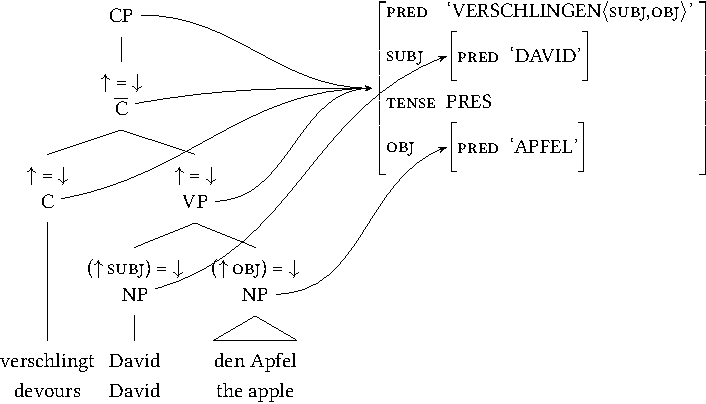
\includegraphics{Figures/verschlingt-david-den-apfel-lfg-lsp-crop}
}
\caption{\label{Abb-Verbstellung-LFG}Analysis of verb placement following \citet[\page 41]{Berman2003a}}
\end{figure}%

{\interfootnotelinepenalty=10%
\noindent
After what we learned about phrase structure rules in Chapters~\ref{Kapitel-PSG} and~\ref{Kapitel-GPSG}, it may seem strange to allow VPs without V. This is not a problem in LFG,
however, since for the analysis of a given sentence, it only has to be ensured that all the necessary parts (and only these) are present. This is ensured by the constraints on 
completeness\is{completeness} and coherence\is{coherence}. Where exactly the information comes from is not important. In Figure~\ref{Abb-Verbstellung-LFG}, the verb information
does not come from the VP, but rather from the C node.
C$'$ is licensed by a special rule:
\ea
\phraserule{C$'$}{
\rulenode{C\\* \up~=~\down}
\rulenode{VP\\*\up~=~\down}}
\z
In LFG rules, there is normally only one element annotated with `\up~=~\down', namely the head. In (\mex{0}), there are two such elements, which is why both equally contribute to the
f"=structure of the mother. The head domain of V has been extended to C. The information about \lfgsubj and \lfgobj comes from the VP and the information about \pred from C.%
\is{head domain!extended|)}\is{verb"=final language}

\section{Local reordering}
\label{Abschnitt-LFG-Umstellung}

Two\is{constituent order} possibilities for treating local reordering have been discussed in the literature:\footnote{%
  \citet[\page 20--21]{Kaplan95a} shows how one can write grammars in the ID/LP format\is{ID/LP grammar} in LFG. A GPSG"=like\indexgpsg analysis of German constituent
  order has not been proposed in the LFG framework.%
}
\begin{itemize}
\item movement of arguments from a base configuration as in GB\indexgb (see \citealp{Choi99a-u})
\item direct licensing by phrase structure rules (see Berman \citeyear[Section~2.1.3.1]{Berman96a-u}; \citeyear{Berman2003a})
\end{itemize}

\noindent
If one assumes that traces are relevant for the semantic interpretation of a given structure, then the first option has the same problems as movement"=based GB analyses.
These have already been discussed in Section~\ref{sec-GB-lokale-Umstellung}.

In what follows, I will present the analysis proposed by  \citet[Section~2.1.3]{Berman96a-u} in a
somewhat simplified form. Case and grammatical functions of verbal arguments are determined
in the lexicon \citep[\page 22]{Berman96a-u}. (\mex{1}) shows the lexical entry for the verb \emph{verschlingen} `devour':\footnote{%
The four cases in German can be represented using two binary features ({\small GOV}, {\small OBL}) \citep[\page 22]{Berman96a-u}. Nominative corresponds to {\small GOV}$-$ and
  {\small OBL}$-$ and accusative to {\small GOV}$+$ and {\small OBL}$-$. This kind of encoding allows one to leave case partially underspecified. If one does not provided a value
  for {\small GOV}, then an element with {\small OBL}$-$  is compatible with both nominative and accusative. Since this underspecification is not needed in the following discussion,
  I will omit this feature decomposition and insert the case values directly.
}$^,$\footnote{%
	Alternative analyses derive the grammatical function of an NP from its case (\citealp[\page 37]{Berman2003a} for German; \citealp[\page 187, \page 201]{Bresnan2001a} for German and Russian\il{Russian}).

\ea
\label{Kasus-Implikation-Berman}
\upshape      (\downsp \case) = \mdacc{} $\Rightarrow$ (\upsp \lfgobj) = \down{}
\z

\noindent
  \citet[Section~2.1]{Karttunen89a-u} makes a similar suggestion for Finnish\il{Finnish} in the framework of Categorial Grammar\indexcxg.
  Such analyses are not entirely unproblematic as case cannot always be reliably paired with grammatical functions. In German, as well as temporal
  accusatives (ii.a), there are also verbs with two accusative objects (ii.b--c) and predicative accusatives (ii.d).

\eal
\ex 
\gll Er arbeitete den ganzen Tag.\\
	 he worked the.\acc{} whole.\acc{} day\\
\ex 
\gll Er lehrte ihn den Ententanz.\\
	 he taught him.\acc{} the.\acc{} duck.dance\\
\ex 
\gll Das kostet ihn einen Taler.\\
	 that costs him.\acc{} a.\acc{} taler\\
\ex 
\gll Sie nannte ihn einen Lügner.\\
	 she called him.\acc{} a.\acc{} liar\\
\zl
All of these accusatives can occur in long"=distance dependencies (see Section~\ref{Abschnitt-NLA-LFG}):

\ea
\gll Wen glaubst du, dass ich getroffen habe.\\
	 who believe you that I met have\\
\glt `Who do you think I met?'
\z

\noindent
\emph{wen} is not the object of \emph{glauben} `believe' and as such cannot be included in the
f"=structure of \emph{glauben} `believe'. One would have to reformulate the implication in
(i) as a disjunction of all possible grammatical functions of the accusative and in addition account
for the fact that accusatives can come from a more deeply embedded f"=structure.

\citet[\page 202]{Bresnan2001a} assumes that nonlocal dependencies crossing a clause involve a gap
in German. With such a gap one can assume that case is only assigned locally within the verbal
projection. In any case one would have to distinguish several types of frontings in German and the
specification of case/grammatical function interaction would be much more complicate than (\ref{Kasus-Implikation-Berman}).%
%Stellt sich aber immer noch die Frage, ob man weiß, was der Trace für kategoriale
%Eigenschaften hat. Man findet den inside out und sagt dann OK, Deine Eigenschaften kenne ich jetzt
%und desahlb muss dann Deine grammatisceh Funktion hier Objekt sein. Oder?
%
% Traces seem to help here, but then there should be a connection between the fronted XP and the
% trace. Is there any connection other than the f-structure? The implication should not apply to the
% prefield. Lots of additional stipulations seem to be needed.
% Bresnan 2001:188 says that Russian does not have traces since it morphologically marks its dependends.
}
\ea
\label{le-verschlingen}
\catlexentry{verschlingt}{V}{(\up\ \pred) = {\small `VERSCHLINGEN\arglist{\lfgsubj, \lfgobj}'}\\*
                             (\up\ \lfgsubj{} {\small AGR CAS}) = NOM\\*
                             (\up\ \lfgobj{} {\small AGR CAS}) = ACC\\*
                             (\up\ \lfgtense) = \small PRES}
\z

%\addlines
\largerpage
\noindent
Berman proposes an analysis that does not combine the verb with all its arguments and adjuncts at
the same time, as was the case in GPSG\indexgpsg. Instead, she chooses the other extreme and assumes
that the verb is not combined with an adjunct or an argument, but rather forms a VP directly. The rule for this is shown in (\mex{1}):
\ea
\label{LFG-v-vp}
\phraserule{VP}{
\rulenode{(V)\\* \up~=~\down}}
\z
At first sight, this may seem odd since a V such as \emph{verschlingen} `devour' does not have the same distribution as a verb with its arguments. However, one should recall that the
constraints pertaining to coherence and completeness of f"=structures play an important role so that
the theory does not make incorrect predictions.
}% footnote breaks

Since the verb can occur in initial position, it is marked as optional in the rule in (\mex{0}) (see Section~\ref{Abschnitt-Verbstellung-LFG}).

The following rule can be used additionally to combine the verb with its subject or object.
\ea
\label{lfg-vp-regel}
\phraserule{VP}{
\rulenode{NP\\* (\upsp \lfgsubj|\lfgobj|\objtheta) = \down}
\rulenode{VP\\* \up~=~\down}}
\z
The `|'\is{$\vert$} here stands for a disjunction\is{disjunction}, that is, the NP can either be the subject or the object of the superordinate f"=structure. Since VP occurs both on the left
and right"=hand side of the rule in (\mex{0}), it can be applied multiple times.
The rule is not complete, however. For instance, one has to account for prepositional objects, for clausal
arguments, for adjectival arguments and for adjuncts. See footnote~\ref{fn-zp} on page~\pageref{fn-zp}.

\largerpage
Figure~\vref{Abb-SOV-LFG} shows the analysis for (\mex{1}a). 
\eal
\ex 
\gll {}[dass] David den Apfel verschlingt\\
      \spacebr{}that David the apple devours\\
\glt `that David is devouring the apple'
\ex 
\gll {}[dass] den Apfel David verschlingt\\
     \spacebr{}that the apple David devours\\
\zl
\begin{figure}
\centerline{%
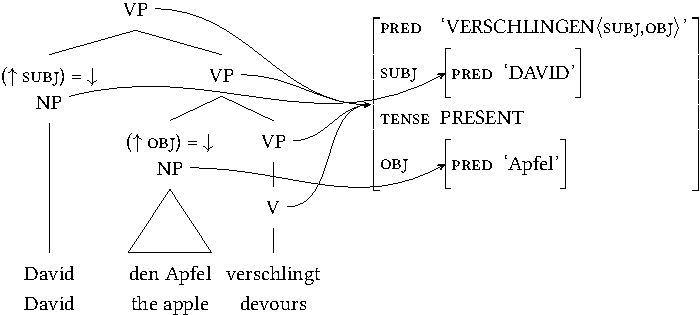
\includegraphics{Figures/david-den-apfel-verschlingt-lfg-lsp-crop}
}
\caption{\label{Abb-SOV-LFG}Analysis of SOV order following \citet{Berman96a-u}}
\end{figure}%
The analysis of (\mex{0}b) is shown in Figure~\vref{Abb-OSV-LFG}.
\begin{figure}
\centerline{%
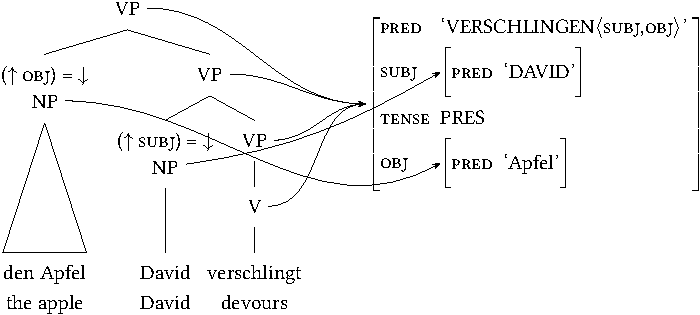
\includegraphics{Figures/den-apfel-david-verschlingt-lfg-lsp-crop}
}
\caption{\label{Abb-OSV-LFG}Analysis of OSV order following \citet{Berman96a-u}}
\end{figure}%
The analysis of (\mex{0}b) differs from the one of (\mex{0}a) only in the order of the replacement
of the NP node by the subject or object.\todostefan{fix the arrows, should not cross SUBJ and OBJ}

One further fact must be discussed: in the rule (\ref{LFG-v-vp}), the verb is optional. If it is
omitted, the VP is empty. In this way, the VP rule in (\ref{lfg-vp-regel}) can have an empty VP on
the right"=hand side of the rule. This VP is also simply
omitted even though the VP symbol in the right-hand side of rule (\ref{lfg-vp-regel})  is not marked as optional.
That is, the corresponding symbol then also becomes optional as a result of taking the rest of the grammar into consideration as well as possible interactions with
other rules.\is{constituent order|)}  

\section{Long"=distance dependencies and functional uncertainty}
\label{Abschnitt-NLA-LFG}

We\is{long"=distance dependency|(} have seen that LFG can explain phenomena such as passivization, local reordering as well as verb placement without transformations.
In Chapter~\ref{Kapitel-GPSG} on GPSG, we already saw that the development of a transformation"=less analysis for long"=distance dependencies constitutes a real achievement.
In LFG, \citet{KZ89a} proposed another transformation"=less analysis of long"=distance dependencies, which we will consider in further detail in what follows.

%\addlines[-1]
In example (\mex{1}), the displaced constituent \emph{Chris} is characterized by two functions:
\ea
\label{ex-Chris-we-think}
Chris, we think that David saw.
\z
For one, it has an argument function which is normally realized in a different position (the \lfgobj function of \emph{saw} in the above example) and additionally it has a discourse function:
a certain emphasis of the information"=structural status in this construction (\textsc{topic} in the matrix clause).
In LFG, \textsc{topic} and \textsc{focus} are assumed to be grammaticalized discourse functions (furthermore, \textsc{subj} is classified as the default discourse function). Only
grammaticalized discourse functions are represented on the level of f"=structure, that is, those
that are created by a fixed syntactic mechanism and that interact with the rest of the syntax. 

Unlike argument functions, the discourse functions  \textsc{topic}\isfeat{topic}\is{topic} and
\textsc{focus}\isfeat{focus}\is{focus} are not lexically subcategorized and are therefore not subject to the completeness\is{completeness} and 
coherence\is{coherence} conditions. The values of discourse function features like \textsc{topic}
and \textsc{focus} are identified with an f"=structure that bears an argument function.  (\mex{1})  
gives the f"=structure for the sentence in (\ref{ex-Chris-we-think}):

\ea
\lfgms{ pred & `THINK\sliste{ \lfgsubj, comp }' \\
        topic & \rnode{topic}{\lfgms{ pred & `CHRIS' \\
                                   }}\\[4mm]
        subj & \lfgms{ pred & `pro'\\
                     }\\
        comp & \lfgms{ pred & `SEE\sliste{ \lfgsubj, \lfgobj }'\\
                       subj & \lfgms{ pred & `DAVID' \\
                                    }\\
                       obj  & \rnode{obj}{}\\
                     }\\
      }
% todo \nodecurve[r]{topic}[r]{obj}{15em}
\nccurve[ncurv=2.2]{topic}{obj}
\z

\noindent
The connecting line means that the value of \textsc{topic} is identical to the value of
\textsc{comp$|$obj}. In Chapter~\ref{chap-feature-descriptions} on feature descriptions, I used boxes for structure sharing
rather than connecting lines, since boxes are more common across frameworks.
It is possible to formulate the structure sharing in (\mex{0}) as an f-structure constraint as in (\mex{1}):
\ea
\label{Topic-Comp-Obj}
(\upsp  \textsc{topic}) = (\upsp \textsc{comp obj})
\z

\noindent
Fronting operations such as (\ref{ex-Chris-we-think}) are possible from various levels of embedding:
for instance, (\mex{1}a) shows an example with less embedding.
The object is located in the same f"=structure as the topic. However, the object in (\ref{ex-Chris-we-think}) comes from a clause embedded under \emph{think}.

The f"=structure corresponding to (\mex{1}a) is given in (\mex{1}b):

\eal
\ex Chris, we saw.
\ex 
\lfgms{ pred & `SEE\sliste{ \lfgsubj, \lfgobj }' \\
        topic & \rnode{topic}{\lfgms{ pred & `CHRIS' \\
                                   }}\\[4mm]
        subj & \lfgms{ pred & `pro'\\
                     }\\
        obj  & \rnode{obj}{}\\
      }
% todo \nodecurve[r]{topic}[r]{obj}{15em}
\nccurve[nodesepA=1pt,ncurv=2.2]{topic}{obj}
\zl

\noindent
The identity restriction for \topic{} and object can be formulated in this case as in (\mex{1}):

\ea
\label{Topic-Obj}
(\upsp  \textsc{topic}) = (\upsp \textsc{obj})
\z

\noindent
Example (\mex{1}a) shows a case of even deeper embedding than in (\ref{ex-Chris-we-think}) and
(\mex{1}b,c) show the corresponding f"=structure and the respective restriction.

\eal
\ex Chris, we think Anna claims that David saw.
\ex 
\lfgms{ pred & `THINK\sliste{ \lfgsubj, comp }' \\
        topic & \rnode{topic}{\lfgms{ pred & `CHRIS' \\
                                   }}\\[4mm]
        subj & \lfgms{ pred & `pro'\\
                     }\\
        comp & \lfgms{ pred & `CLAIM\sliste{ \lfgsubj, comp }\\
                       subj & \lfgms{ pred & `ANNA' \\
                                   }\\
                       comp & \lfgms{ pred & `SEE\sliste{ \lfgsubj, \lfgobj }\\
                                      subj & \lfgms{ pred & `DAVID' \\
                                                   }\\
                                      obj  & \rnode{obj}{}\\
                                    }\\
                     }\\
      }
% todo \nodecurve[r]{topic}[r]{obj}{15em}%
\nccurve[ncurv=2.2]{topic}{obj}
\ex\label{Topic-Comp-Comp-Obj}
(\upsp  \textsc{topic}) = (\upsp \textsc{comp comp obj})
\zl


\noindent
The restrictions in (\ref{Topic-Comp-Obj}), (\ref{Topic-Obj}) and
(\ref{Topic-Comp-Comp-Obj}) are c"=structure constraints. The combination of a c"=structure with (\ref{Topic-Comp-Obj}) is given in (\mex{1}):
\ea
\begin{tabular}[t]{@{}ccc@{~=~}lc@{}}
CP & $\rightarrow$ & \multicolumn{2}{l}{\hspaceThis{(\upsp \textsc{topic})}XP} & C$'$ \\
 & &  (\upsp \textsc{topic}) & \down & \up~=~\down \\
 & &  (\upsp \textsc{topic}) & (\upsp \textsc{comp obj})\\
\end{tabular}
\z
\addlines
(\mex{0}) states that the first constituent contributes to the \textsc{topic} value in the f"=structure of the mother and furthermore that this topic value has to be
identical to that of the object in the complement clause. We have also seen examples of other embeddings of various depths. We therefore need restrictions
of the following kind as in (\mex{1}): 
\eal
\ex (\upsp  \textsc{topic}) = (\upsp \textsc{obj})
\ex (\upsp  \textsc{topic}) = (\upsp \textsc{comp obj})
\ex (\upsp  \textsc{topic}) = (\upsp \textsc{comp comp obj})
\ex \ldots
\zl
The generalization emerging from these equations is given in (\mex{1}):
\ea
(\upsp  \textsc{topic}) = (\upsp \textsc{comp* obj})
\z

\noindent
Here, `*'\is{*} stands for an unrestricted number of occurrences of \mbox{\small COMP}. This means of leaving the possible identification of discourse and grammatical function open is known
as \emph{functional uncertainty}\is{functional uncertainty}, see \citew{KZ89a}.

As was shown in the discussion of examples (\ref{bsp-fronted-focus}) and (\ref{bsp-fronted-topic}) on
page~\pageref{bsp-fronted-focus}, it is not the case that only a \textsc{topic} can be placed in the specifier position of CP in English as \focus can occur there too.
One can use disjunctions in LFG equations and express the corresponding condition as follows:

\ea
(\upsp  \textsc{topic$|$focus}) = (\upsp \textsc{comp* obj})
\z
One can introduce a special symbol for \textsc{topic$|$focus}, which stands for a disjunction of discourse functions: \textsc{df}\isfeat{df}.
(\mex{0}) can then be abbreviated as in (\mex{1}):

\ea
(\upsp  \textsc{df}) = (\upsp \textsc{comp* obj})
\z

\noindent
The final version of the c"=structure rule for fronting in English will therefore have the form of
(\mex{1}):\footnote{%
  Note that the two disjunctions that are abbreviated by the respective occurrences of \textsc{df}
  are independent in principle. This is unwanted. We want to talk about either a topic or a focus
  not about a topic and a focus in the mother f-structure. So additional machinery is needed to
  ensure that both occurrences of \textsc{df} refer to the same discourse function.
}
\ea
\begin{tabular}[t]{@{}ccc@{~=~}lc@{}}
CP & $\rightarrow$ & \multicolumn{2}{l}{\hspaceThis{(\upsp \textsc{df})}XP} & C$'$ \\
 & &  (\upsp \textsc{df}) & \down & \up~=~\down \\
 & &  (\upsp \textsc{df}) & (\upsp \textsc{comp* obj})\\
\end{tabular}
\z
In German, as well as objects, nearly any other constituent (\eg subjects, sentential complements, adjuncts) can be fronted. The c"=structure rule for
this is shown in
(\mex{1}):\footnote{\label{fn-zp}%
  \citet{Berman96a-u} uses the symbol ZP for symbols in the prefield rather than XP in (\mex{1}). She formulates various phrase structure rules for ZPs, which replace ZP
  with NP, PP, AP and various adjuncts. Following Berman, ZPs can also be combined with the verb in the middle field. For reasons of exposition, I refrained from using 
  ZP symbols in the formulation of the VP rule (\ref{lfg-vp-regel}) in Section~\ref{Abschnitt-LFG-Umstellung} and instead used NP directly.
}
\ea
\begin{tabular}[t]{@{}ccc@{~=~}lc@{}}
CP & $\rightarrow$ & \multicolumn{2}{l}{\hspaceThis{(\upsp \textsc{df})}XP} & C$'$ \\
 & &  (\upsp \textsc{df}) & \down & \up~=~\down \\
 & &  (\upsp \textsc{df}) & (\upsp \textsc{comp* gf})\\
\end{tabular}
\z
Here, \textsc{gf} is an abbreviation for a disjunction of grammatical functions which can occur in the prefield.
\is{long"=distance dependency|)}



\section{Summary and classification}

LFG is a constraint"=based theory and utilizes feature descriptions and PSG rules. Grammatical functions are treated
as primitives of the theory, which sets LFG apart from most of the other theories covered in this book. They are not defined structurally (as in GB). LFG is a lexicalist theory. Like GPSG, LFG can do without transformations. Processes affecting
argument structure such as passivization are analyzed by means of lexical rules. Whereas GPSG treated long"=distance dependencies using the percolation of information
in trees, LFG uses functional uncertainty: a part of the f"=structure is identified with another
f"=structure that can be embedded to an arbitrary depth. Coherence\is{coherence} and completeness\is{completeness}
ensure that the long"=distance dependency can be correctly resolved, that is, it ensures that a fronted object is not assigned to an f"=structure which already contains an object or one
in which no object may occur.

While LFG does contain a phrase"=structural component, this plays a significantly less important role compared to other models of grammar. There are rules in which all constituents are
optional and it has even been proposed for some languages that there are rules where the part of speech of the constituents is not specified (see Section~\ref{sec-Diskussion-X-Bar}).
In these kinds of grammars, f"=structure, coherence and completeness work together to ensure that the grammar only allows well"=formed structures.

LFG differs from other theories such as \hpsg and variants of \cxg in that feature structures are untyped. Generalizations can therefore not be represented in type hierarchies. 
Until a few years ago, the hierarchical organization of knowledge in inheritance hierarchies\is{inheritance} did not form part of theoretical analyses. In computer implementations,
there were macros\is{macro} but these were viewed as abbreviations without any theoretical status. It is possible to organize macros into hierarchies and macros were discussed explicitly
in \citew*{DKK2004a} with reference to capturing linguistic generalizations. \citet*{ADT2008a} suggest using macros not only for the organization of lexical items but also for
capturing generalizations regarding c"=structure annotations. Because of these developments, there was a greater convergence between LFG and other theories such as HPSG and CxG.

\citet{Williams84a} compares analyses in LFG with GB. He shows that many analyses are in fact transferable: the function that f"=structure has in LFG is handled by the
Theta"=Criterion\is{theta-theory@$\theta$-Theory}\is{theta-criterion@Theta"=Criterion} and Case Theory\is{case}\is{Case Theory} in GB. LFG can explicitly differentiate between subjects and non"=subjects. In GB, on the other hand,
a clear distinction is made between external\is{argument!external} and internal\is{argument!internal} arguments (see \citealp[Section~1.2]{Williams84a}). In some variants of GB, as well as
in HPSG\indexhpsg and CxG\indexcxg, the argument with subject properties (if there is one) is marked explicitly \citep{Haider86,HM94a,Mueller2003e,MR2001a}. This special argument
is referred to as the \emph{designated argument}\is{argument!designated}. In infinitival constructions, subjects are often not expressed inside the infinitival phrase. Nevertheless, 
the unexpressed subject is usually coreferential with an argument of the matrix verb:

\eal
\ex 
\gll Er versucht, [das Buch zu lesen].\\
	 he tries \spacebr{}the book to read\\
\glt `He is trying to read the book.'
\ex 
\gll Er zwingt ihn, [das Buch zu lesen].\\
	 he forces him \spacebr{}the book to read\\
\glt `He is forcing him to read the book.´
\zl 
This is a fact that every theory needs to be able to capture, that is, every theory must be able to differentiate between subjects and non"=subjects.

For a comparison of GB/Minimalism and LFG/HPSG, see \citew{Kuhn2007a}.

 
\questions{

\begin{enumerate}
\item What do the terms \emph{coherence} and \emph{completeness} mean?
\item What are extended head domains?
\item What does lexical integrity mean?
\end{enumerate}

\vspace*{1cm}
}

\exercises{

\begin{enumerate}
\item Give the lexical entry for \emph{kannte} `knew'.
\item How could one analyze the following sentence?
\ea
\gll Den Apfel verschlingt David.\\
	 the apple devours David\\
\glt `David devours the apple.'
\z
Provide the necessary c"=structure rules. What kind of f"=structure is licensed?
Draw a syntactic tree with corresponding references to the f"=structure. For fronted constituents,
simply write NP rather than expanding the XP node.
The c"=structure rule for the NP can also be omitted and a triangle can be drawn in the tree.
\end{enumerate}

\vspace*{1cm}
}

\clearpage 
\furtherreading{
Section~\ref{Abschnitt-Format-LFG} was based extensively on the textbook and introductory article of \citet{Dalrymple2001a-u,Dalrymple2006a}. Additionally, I have drawn from
teaching materials of Jonas Kuhn from 2007. \citew{Bresnan2001a} is a comprehensive textbook in English for the advanced reader. Some of the more in"=depth analyses of
German in LFG are \citew{Berman96a-u,Berman2003a}.  \citew{SdA2016a-u} is an introduction to LFG that uses French\il{French} examples. The authors demonstrate how the XLE system can be used for the development of a
French\il{French} LFG grammar. The textbook also discusses the Finite State Morphology component that comes
with the XLE system.

\citet{Levelt89a} developed a model of language production based on LFG.
 \citet{Pinker84a-u} -- one of the best"=known researchers on language acquisition -- used LFG as the model for his theory of acquisition. For another theory on first and second
 language acquisition that uses LFG, see \citew{Pienemann2005a}. 
}


%      <!-- Local IspellDict: en_US-w_accents -->



%% Bresnan:

%% The internal structure of a language represents the meaningful grammatical relations of sentences (how their syntactic functions are associated with semantic predicate argument relations); this structure is determined by generalizations about case government, pronominal binding, and agreement relations among the predicators and arguments of a sentence. The principle of universality states that internal structures are largely invariant across languages. The formal model of internal structure in LFG is the f-structure, 'functional structure'. (1996:34 f.)

%% As we have already seen in Ch. 3, the principles of completeness and coherence require full
%% representation of grammatical relations in f-structure. Full representation might be thought of
%% as a universal iconicity requirement between syntax and semantics at f-structure. (1996:83) 


% Dyvik dazu: http://folk.uib.no/hfohd/LFG99/LFG99Dyvik.html
